\documentclass{article}
\usepackage{graphicx}
\usepackage{wrapfig}
\usepackage{titling}
\usepackage[swedish]{babel}
\usepackage{subcaption}
\usepackage{caption}
\usepackage{ulem}
\usepackage{emoji}

\usepackage[a4paper, total={13cm, 20cm}, top = 5cm, left=1.5cm, right=2cm]{geometry}

\title{Rengöring av Ice^3}
\author{Julia Karlsson, Källarmästare}
\date{2023}

\setlength{\droptitle}{-3.6cm}
\begin{document}

\maketitle{}


\begin{wrapfigure}[3]{r}{0.3\textwidth}
    \raggedright
    \vspace{-6cm}
    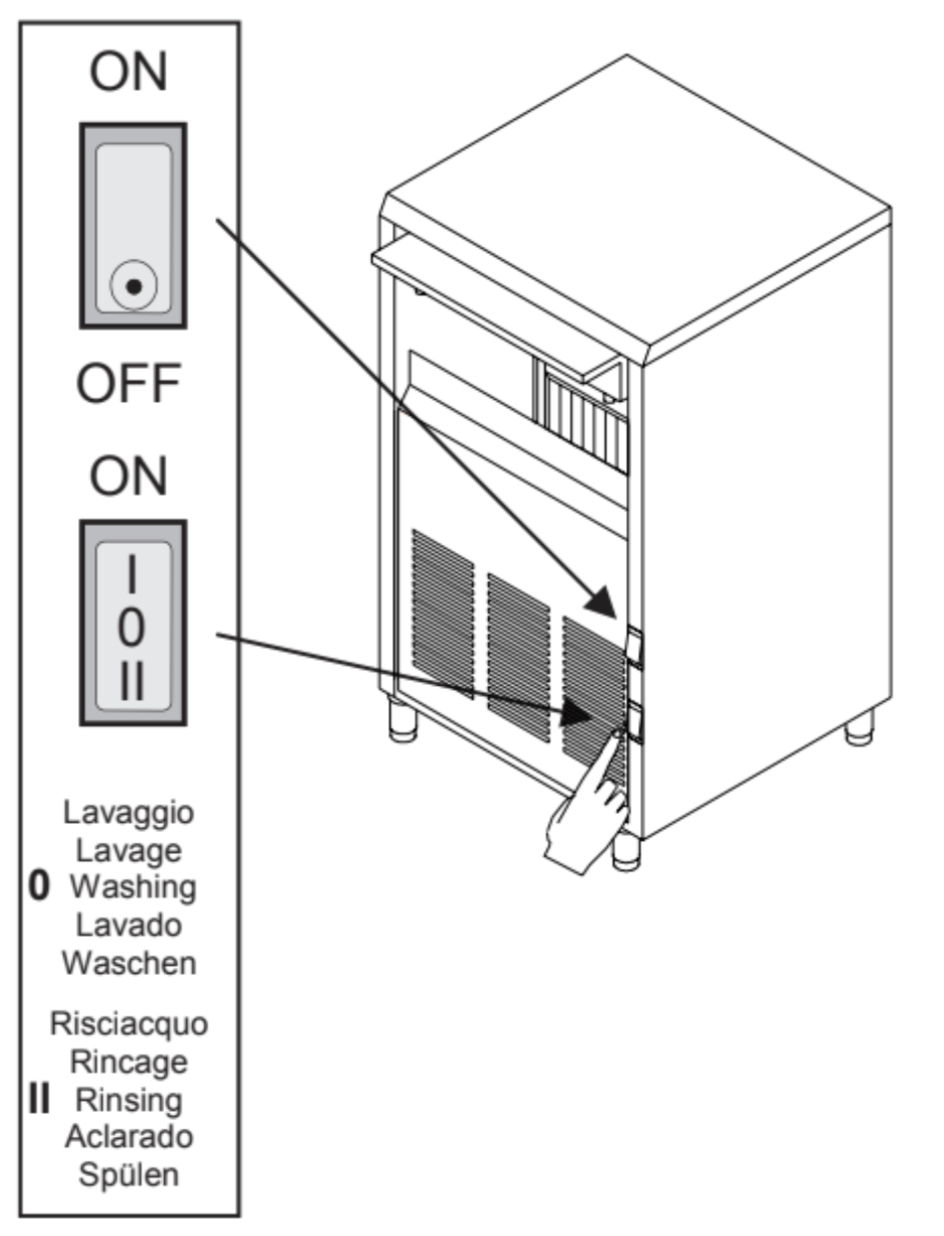
\includegraphics[width=0.4\textwidth]{bilder/1.png}
    \vspace{-3.1cm}
    \caption*{\qquad \qquad \qquad \qquad  \quad \mbox{Steg 1: Knappar}}
\end{wrapfigure}



\section*{What do?}
\subsection*{Steg 1:}
Put cleaning switch on rinsing position and make sure that all ice cubes have been released from their cups. \\ Byt till läge II på den nedre knappen, vänta tills alla kuber lossnat från sin kopp. 

\begin{wrapfigure}[4]{r}{0.19\textwidth}
    \raggedright
    \vspace{-2cm}
    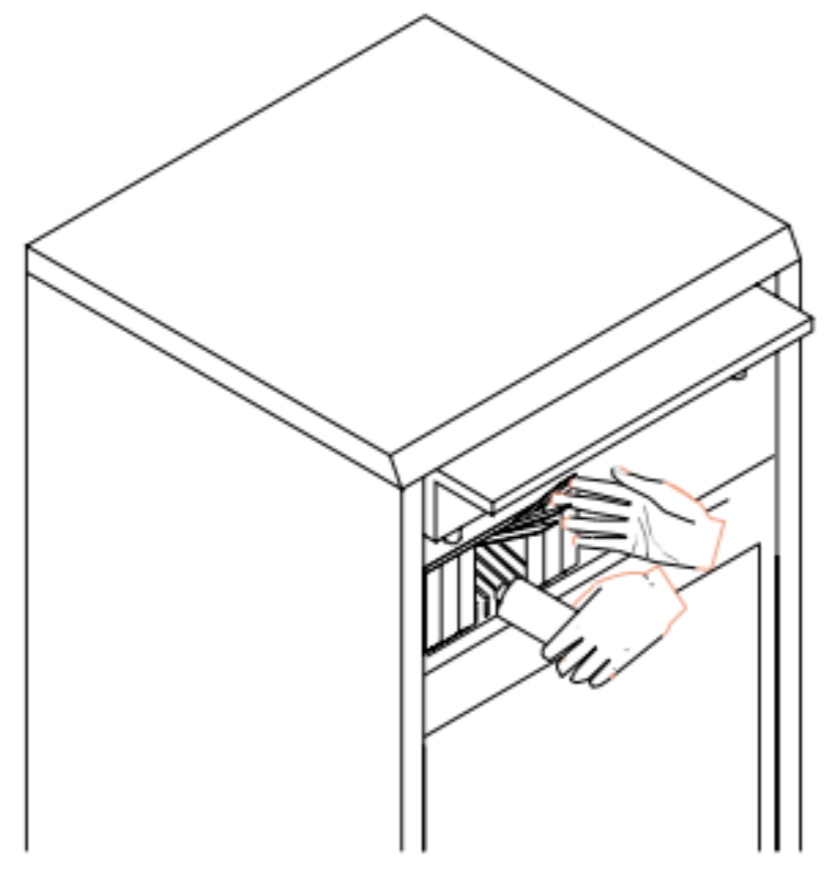
\includegraphics[width=0.28\textwidth]{bilder/2.png}
    \caption*{\hspace{1.5cm} Steg 2}
\end{wrapfigure}



\subsection*{Steg 2:}
Put cleaning switch (see top figure) in washing position and fill 0,5 liters of white vinegar in water reserve. Wait for approx \emph{30 minutes}. \\ Sätt den nedre knappen (bild 3.1) till läge 0, sätt 0,5 liter 6\%-ig ättika i vattenreserven. Vänta ca \emph{30 minuter}. 



\subsection*{Steg 3:}

Switch off main switch, then remove flap support (the metal board above the flaps, attached with 2 large screws), grid and overflow pipe (on the right in the reserve, pull straight up) according to pictures 3.1--3.4. Wait until liquid has drained. \\ Stäng av på övre knappen, och ta sedan bort flärparna (skruva lös metallplattan ovanför flärparna), gallerhyllan innanför och ''spillröret'' (till höger, dra rakt upp, skruvas inte). Se bilder 3.1--3.4 för referens. Vänta tills vätskan runnit ut.



% \vspace{2em}
% \hspace{-1.5cm} 
% 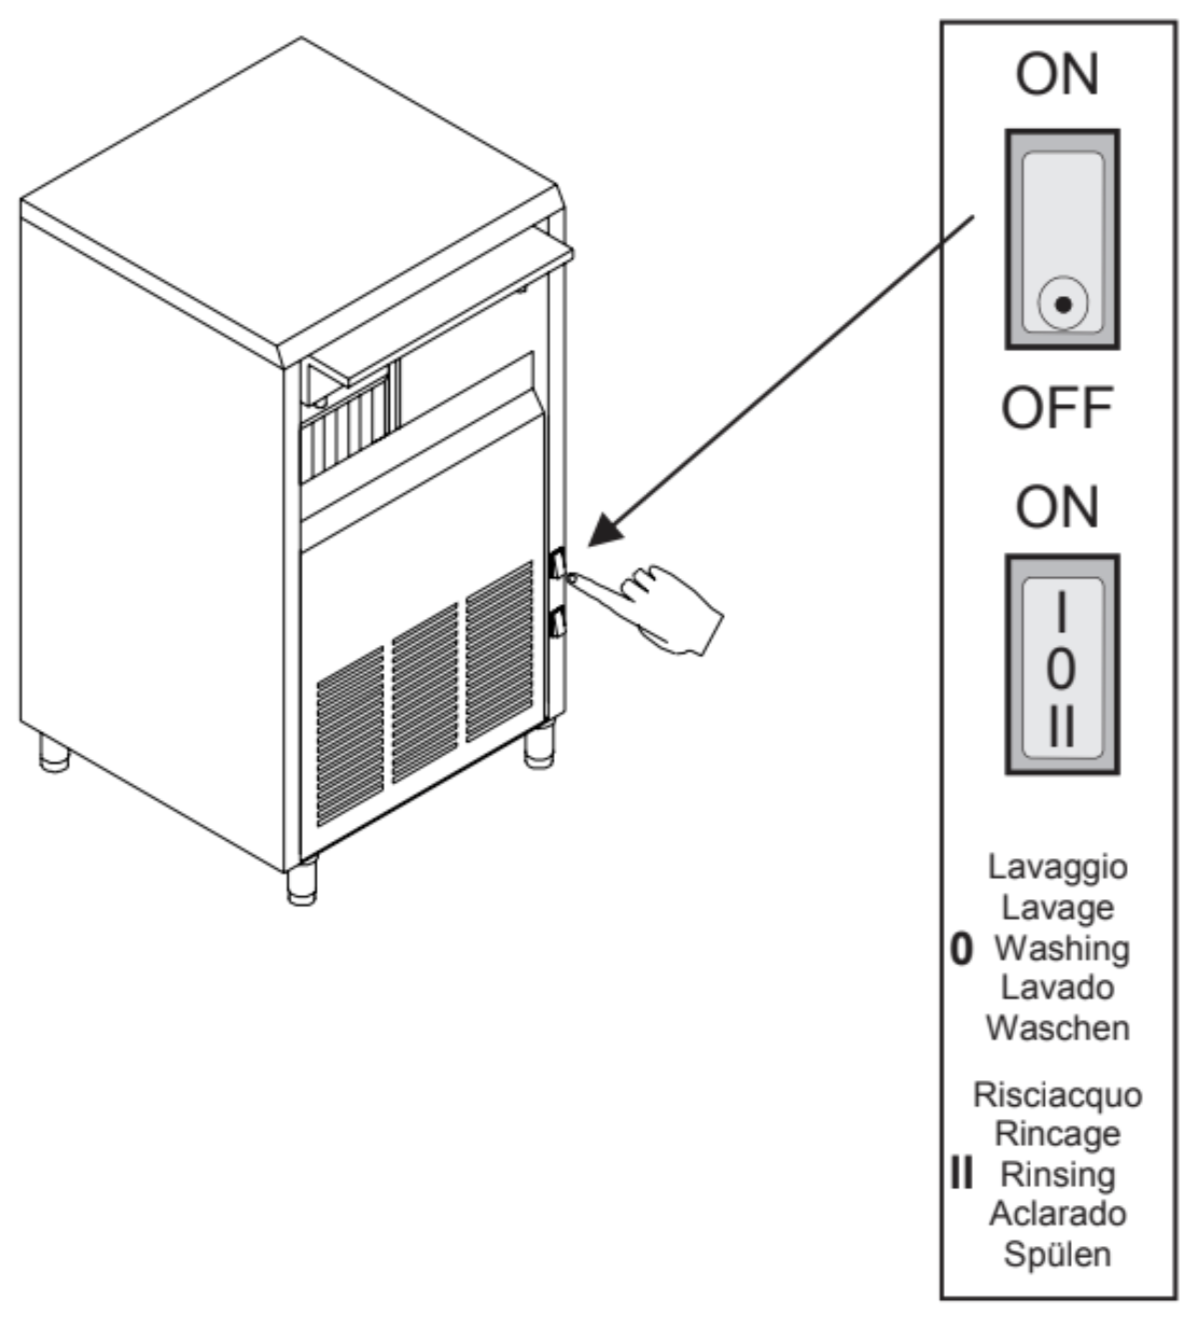
\includegraphics[height=0.4\textwidth]{bilder/3.png}
% 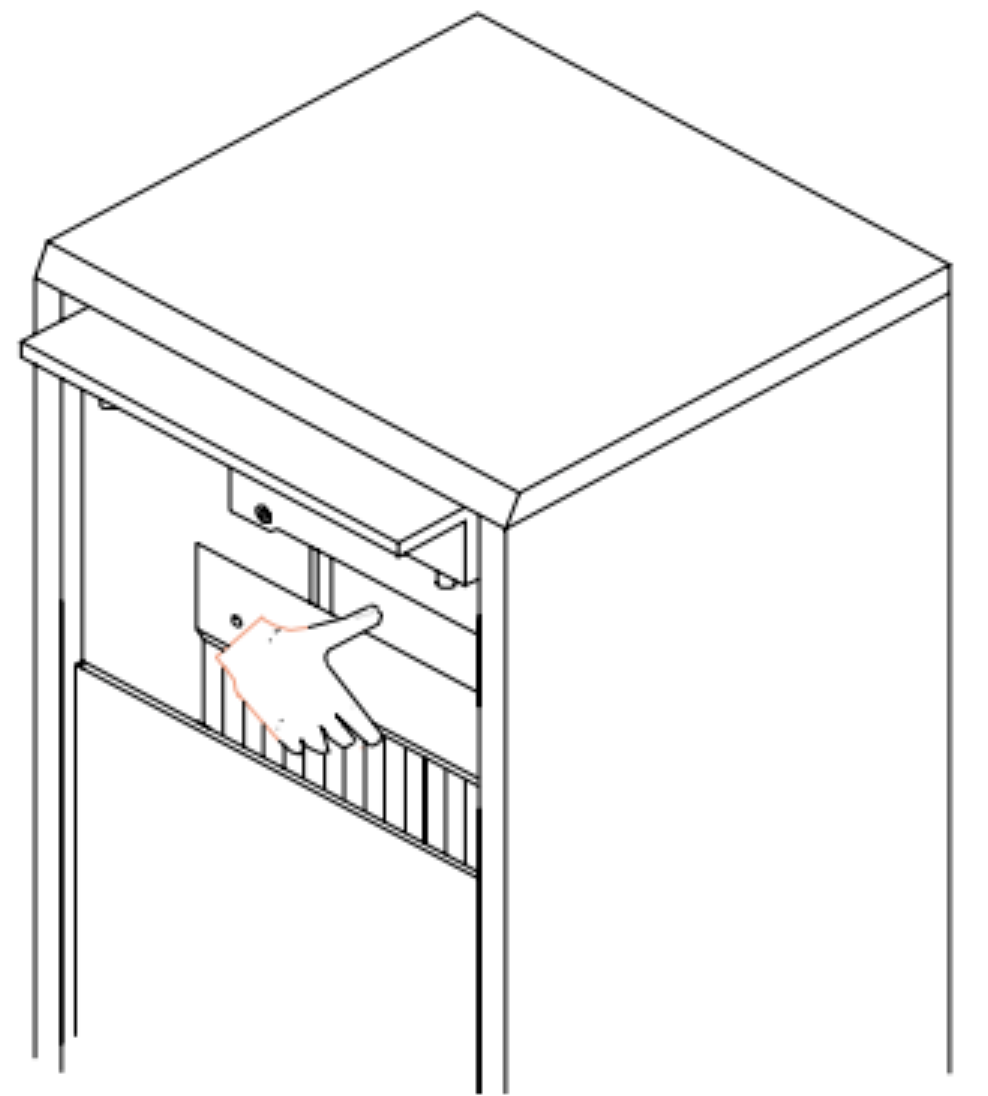
\includegraphics[height=0.3\textwidth]{bilder/4.png}
% 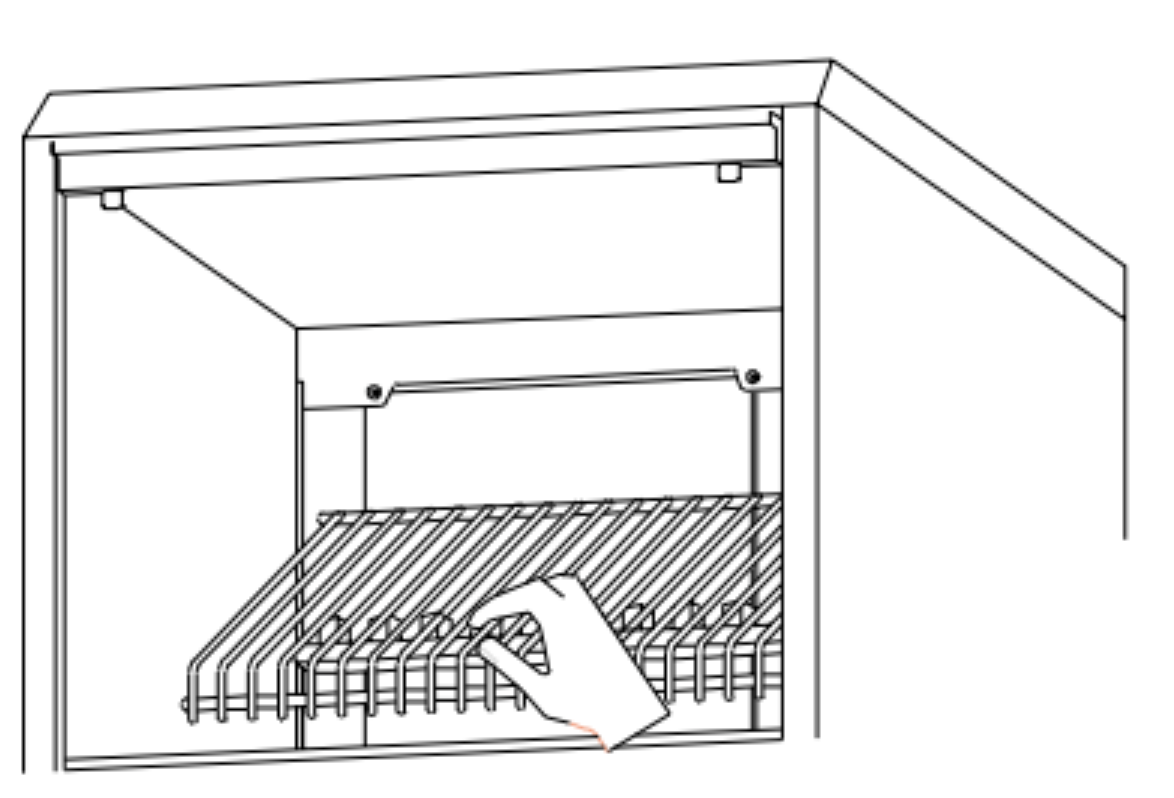
\includegraphics[height=0.3\textwidth]{bilder/5.png} 
% \vspace{-5px}




%%%

\vspace{2em}
\begin{figure}[h!]
    \centering
    \hspace{-0.5cm} 
    \begin{subfigure}[t]{0.3\textwidth}
        \centering
        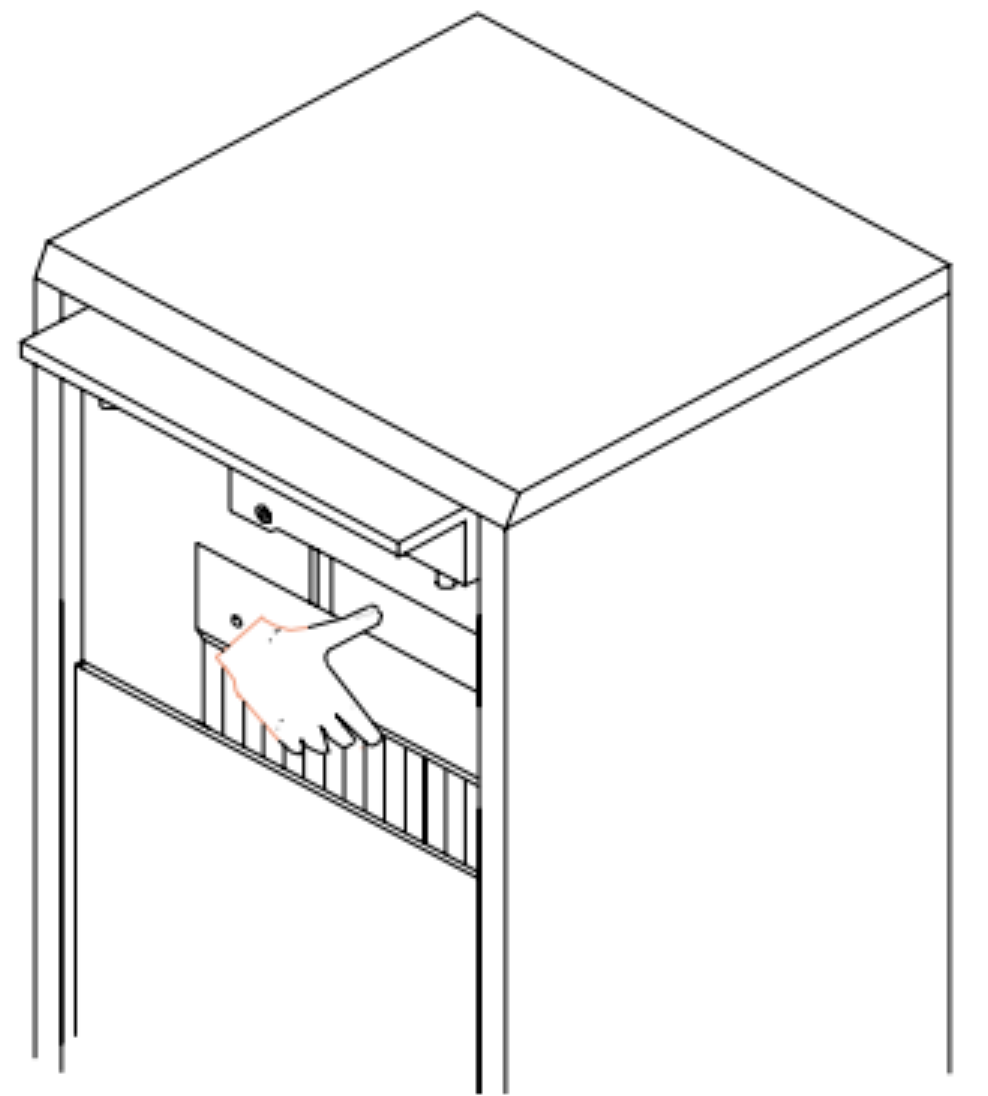
\includegraphics[width=\linewidth]{bilder/4.png}
        \caption*{Steg 3.1}
    \end{subfigure}
    \hfill
    \hspace{-1cm} 
    \begin{subfigure}[t]{0.3\textwidth}
        \centering
        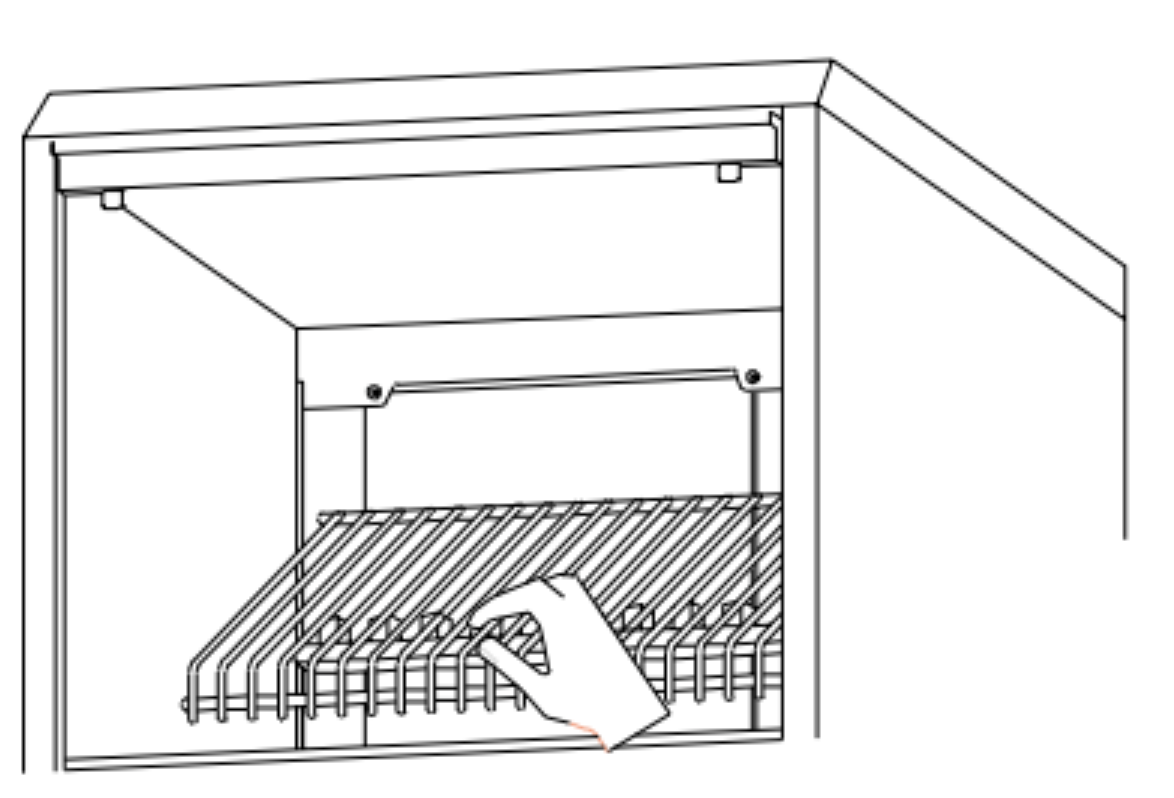
\includegraphics[width=1.2\linewidth]{bilder/5.png}
        \caption*{Steg 3.2}
    \end{subfigure}
    \hfill
    \begin{subfigure}[t]{0.3\textwidth}
        \centering
        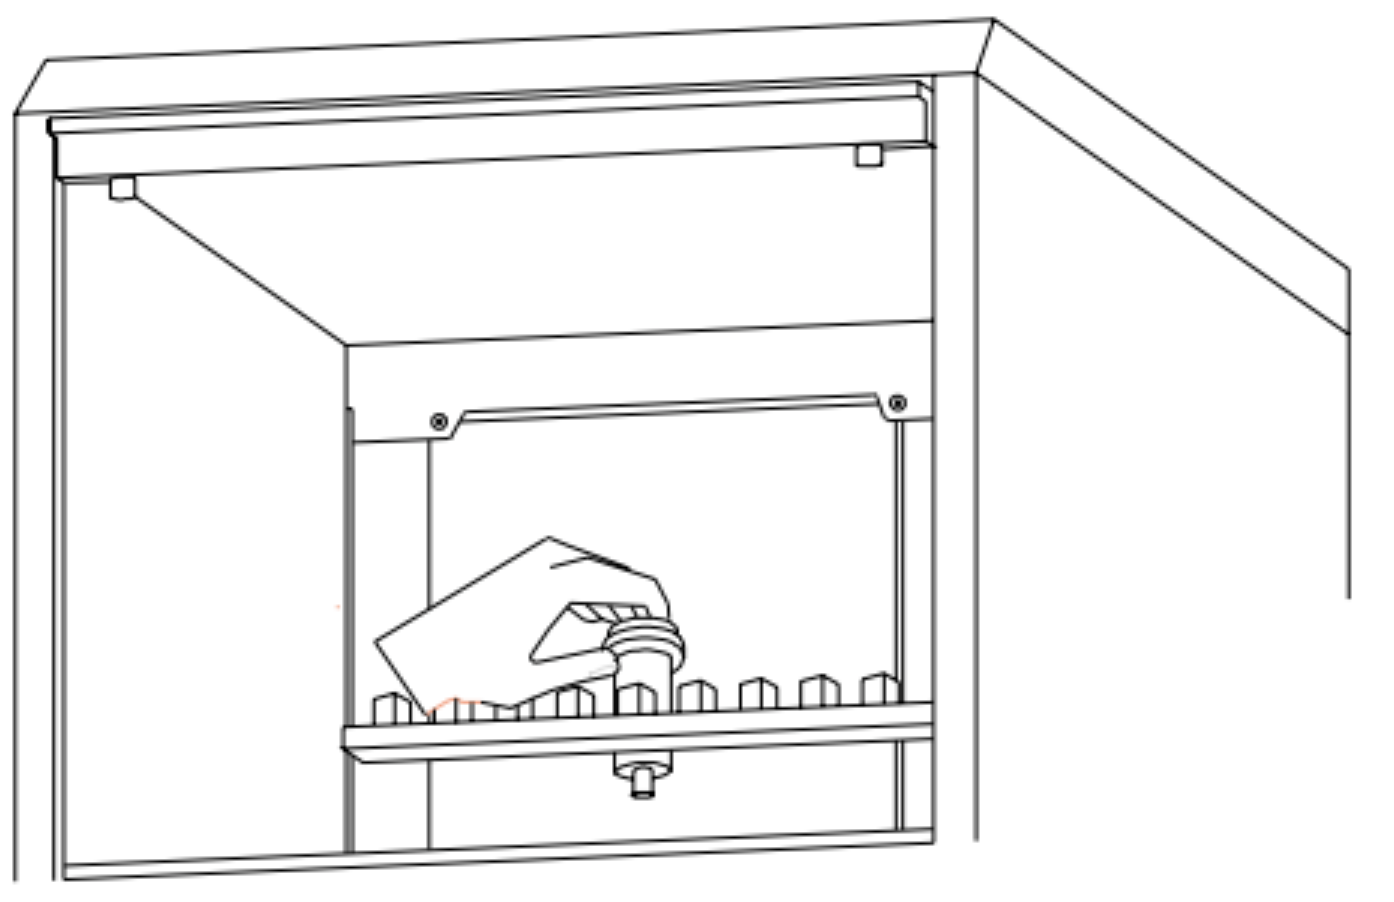
\includegraphics[width=1.2\linewidth]{bilder/6.png}
        \caption*{Steg 3.3}
    \end{subfigure}
\end{figure}

\newpage
\newgeometry{top=3cm}


\subsection*{Steg 4:}

Clear and clean sprayer arm and jets. The arm is only attached in the back through the hose, pull straight out, holding the hose (part of it should come with). Rotate spray jets as shown (4.2). Clean water suction \sout{filter}pipe of the pump. Put everything back. \\ Ta bort och rengör sprejarm och vattensprutor. Sprejarmen sitter endast fast bak i maskinen genom slangen, dra den rakt ut. Håll i slangen, en del av den ska komma med. Rotera vattensprejarna enligt bild 4.2. Rengör inlopps\sout{-filtret}röret som sitter fast.

% 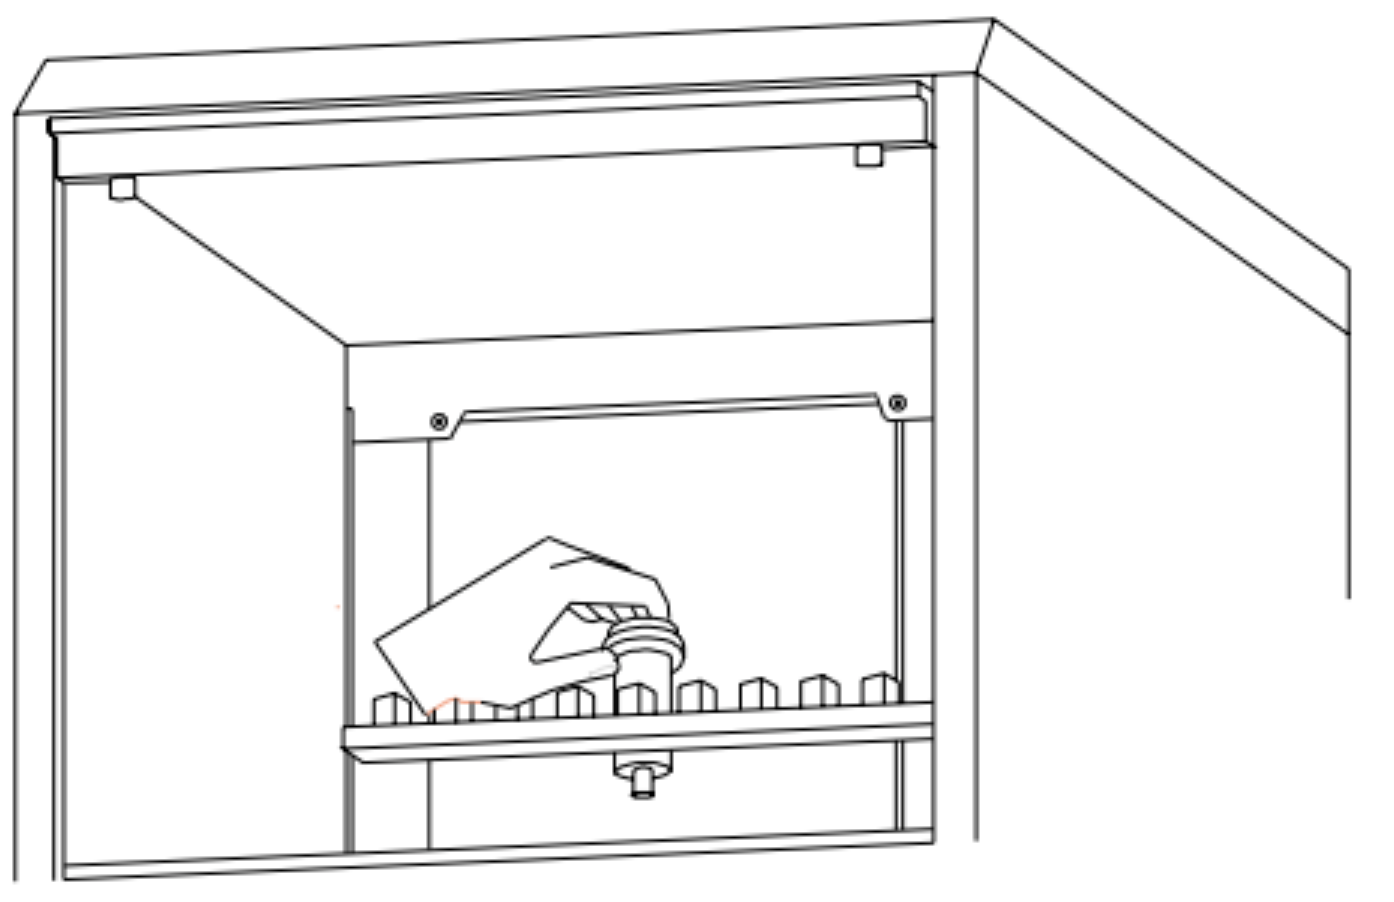
\includegraphics[width=0.45\textwidth]{bilder/6.png}
% 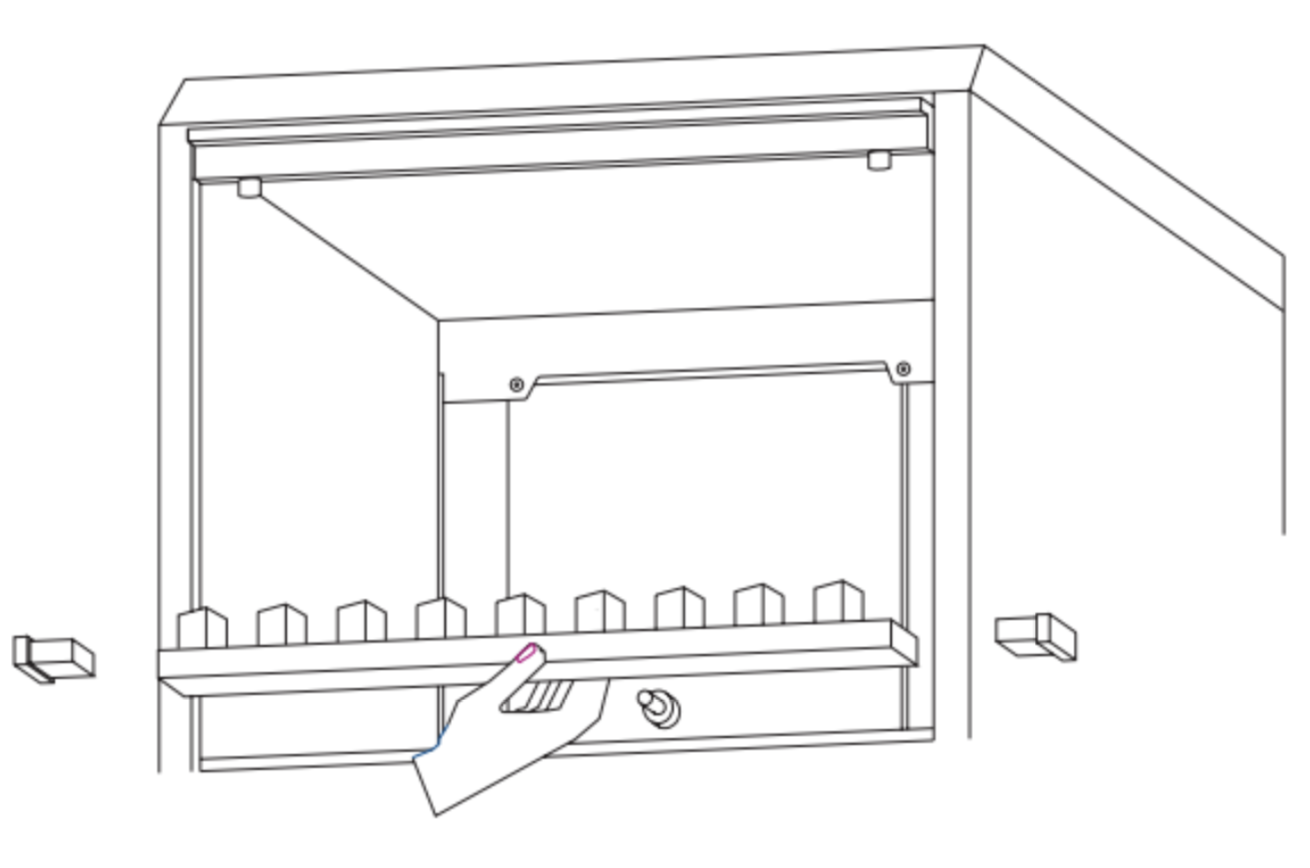
\includegraphics[width=0.45\textwidth]{bilder/7.png} \\
% 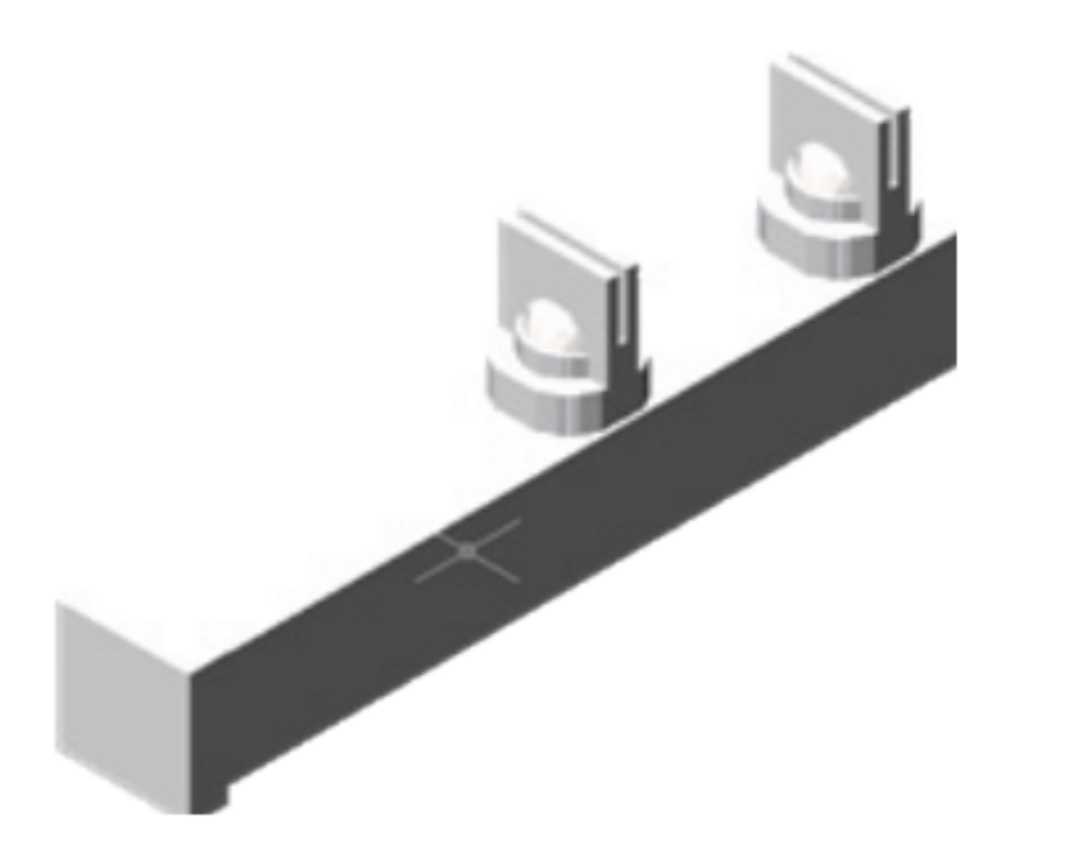
\includegraphics[width=0.45\textwidth]{bilder/8.png}
% 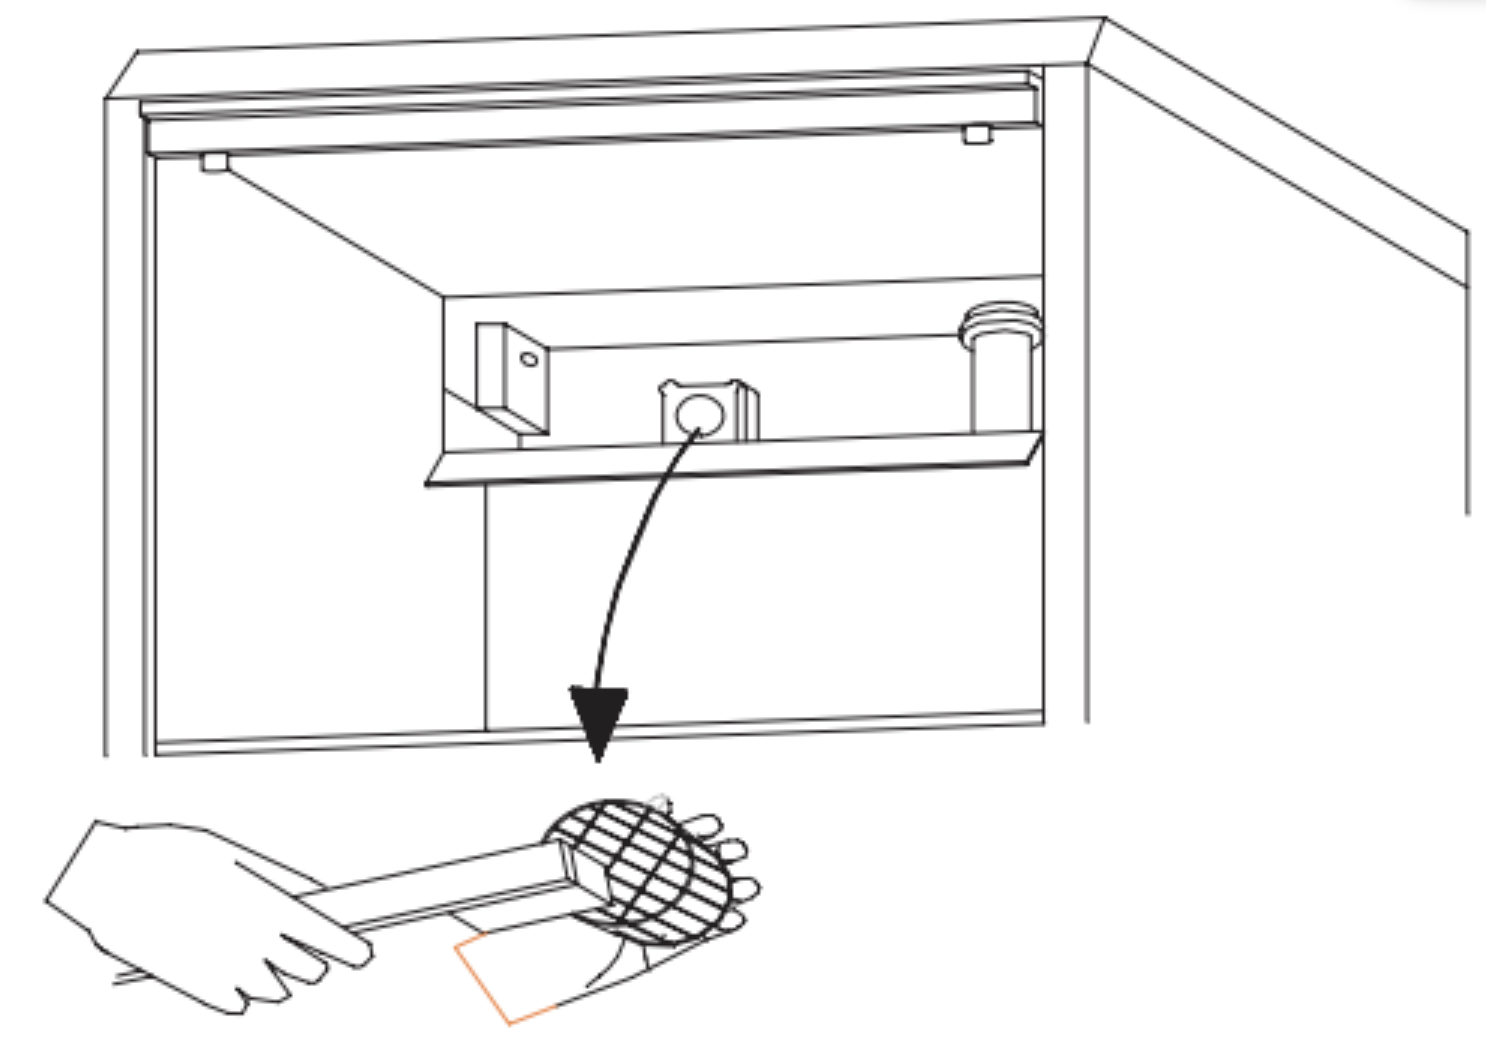
\includegraphics[width=0.45\textwidth]{bilder/9.png} \\

%%%%%%

\begin{figure}[h!]
    \centering
    \begin{subfigure}[t]{0.45\textwidth}
        \centering
        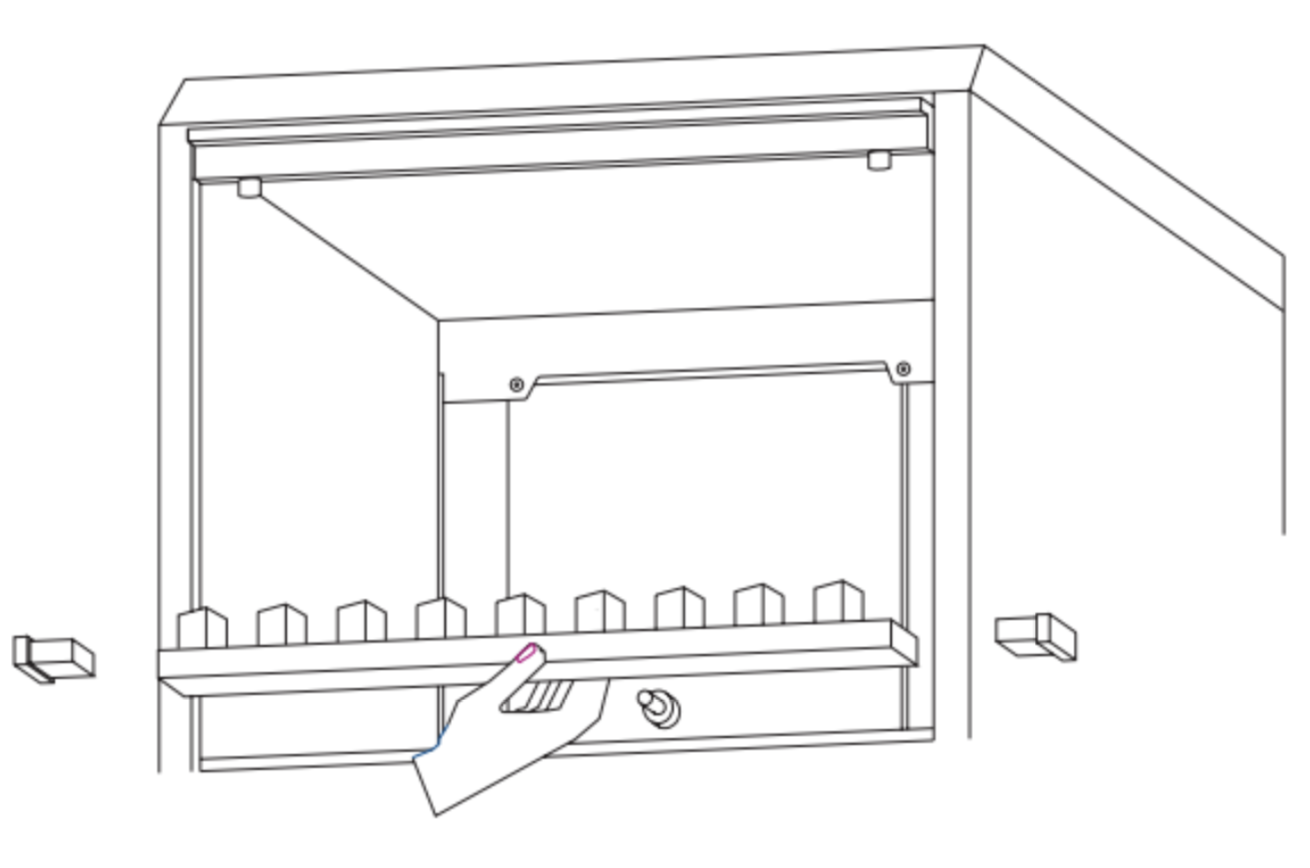
\includegraphics[width=1.1\linewidth]{bilder/7.png}
        \caption*{Steg 4.1: Arm}
    \end{subfigure}
    \hfill
    \begin{subfigure}[t]{0.45\textwidth}
        \centering
        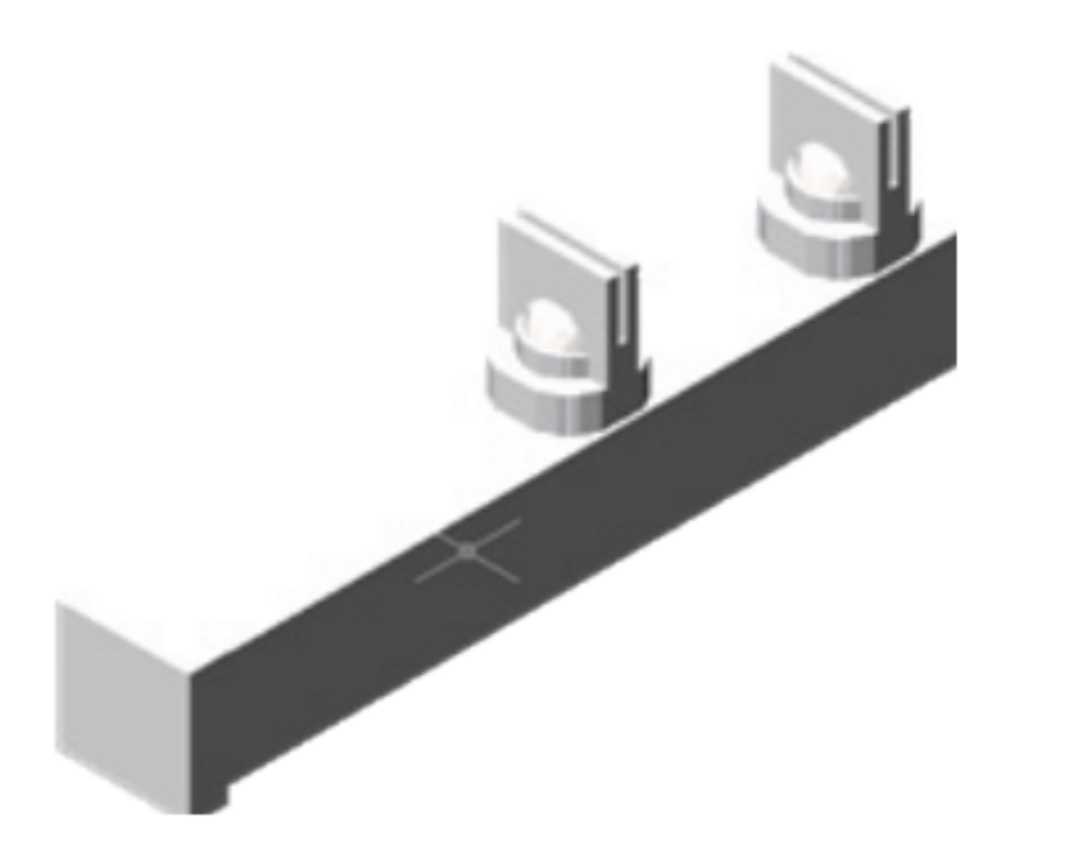
\includegraphics[width=\linewidth]{bilder/8.png}
        \caption*{Steg 4.2: Riktning på vattensprejarna \\ Spray jet rotation}
    \end{subfigure}
    \hfill
    \vspace{0.3cm}
    \begin{subfigure}[t]{0.45\textwidth}
        \centering
        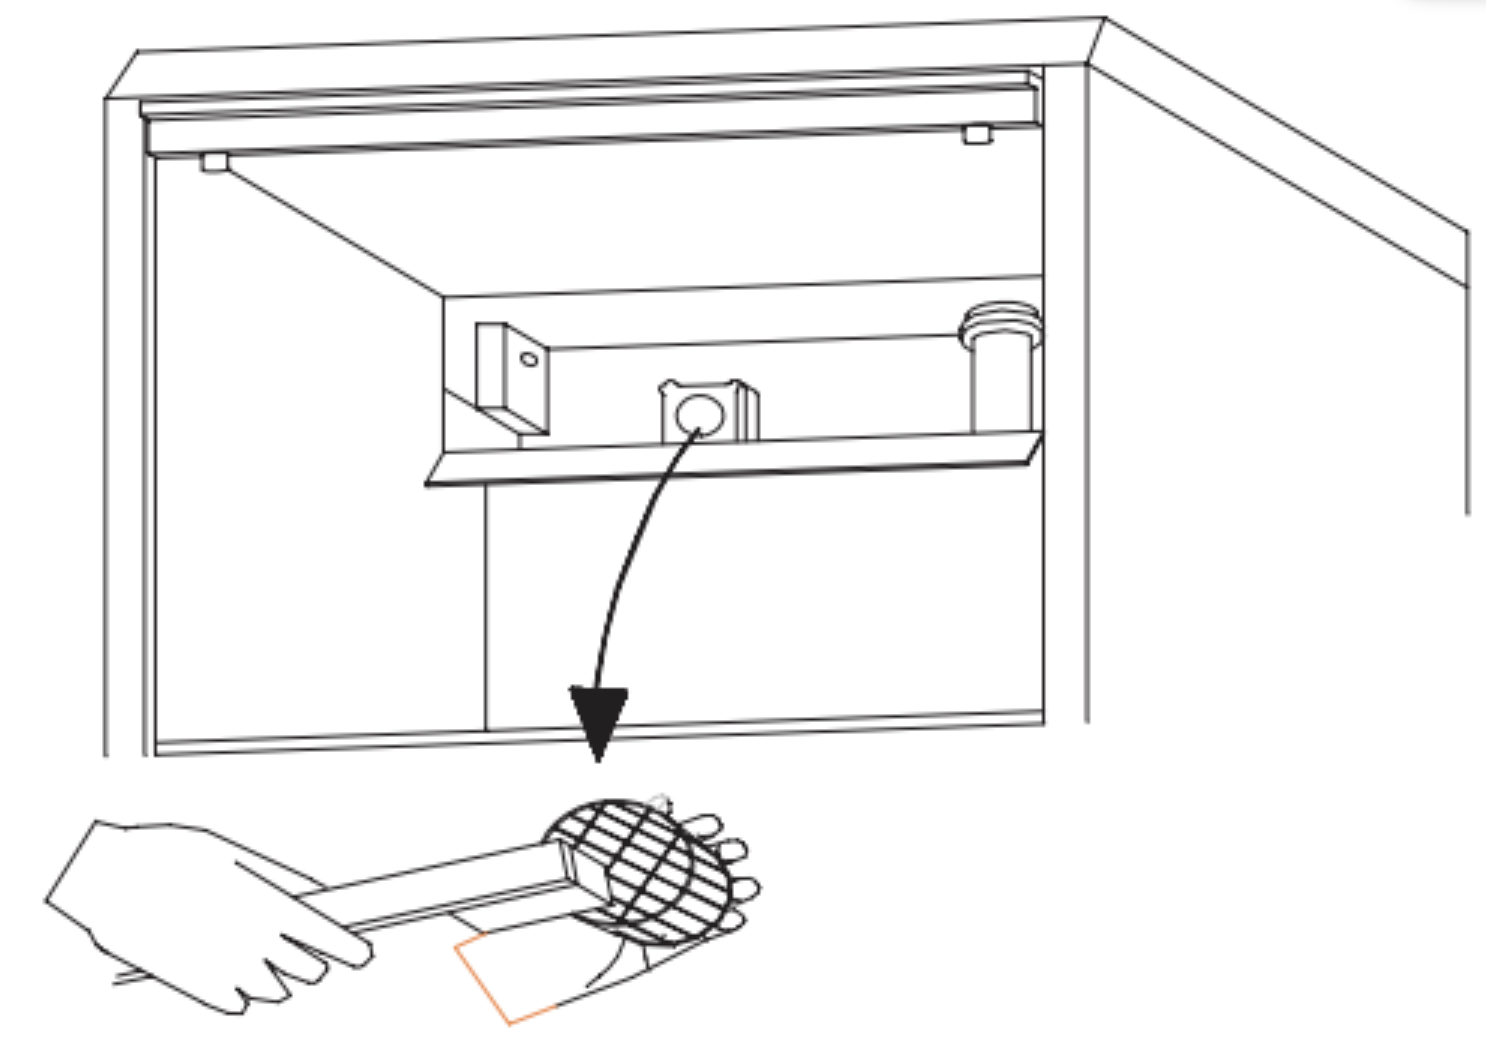
\includegraphics[width=\linewidth]{bilder/9.png}
        \caption*{Steg 4.3: Inloppsrör $||$ Water suction pipe}
    \end{subfigure}
\end{figure}



\subsection*{Steg 5:}
Put overflow pipe, grid and flap support in original position. \\ Sätt tillbaka röret, gallret och flärparna på sin plats igen.

\subsection*{Steg 6:}
Put cleaning switch (lower) in rinsing position, switch on main switch (upper) and \emph{wait 25 minutes}. \\ Byt till läge 2 (rinsing) på nedre knappen, sätt på övre knappen, och \emph{vänta 25 minuter}.

\subsection*{Steg 7 (sista steget!):}
Put cleaning switch (lower) on working position ‘ON’. \\ Byt till läge 1 (ON) på nedre knappen!! \\

\centering
\textbf{Wowie vilken kämpe! Slay \emoji{sparkles} du är klar :) }

\end{document}
